\subsection*{Pinning}
Host data allocations are pageable by default which means that the GPU cannot access data directly from pageable host memory. When a data transfer from pageable host memory to device memory is invoked, the CUDA driver must first allocate a pinned host array, copy the host data to the pinned array, and then transfer the data from the pinned array to device memory\cite{transfer}, as illustrated below.
\begin{figure}[H]\centering
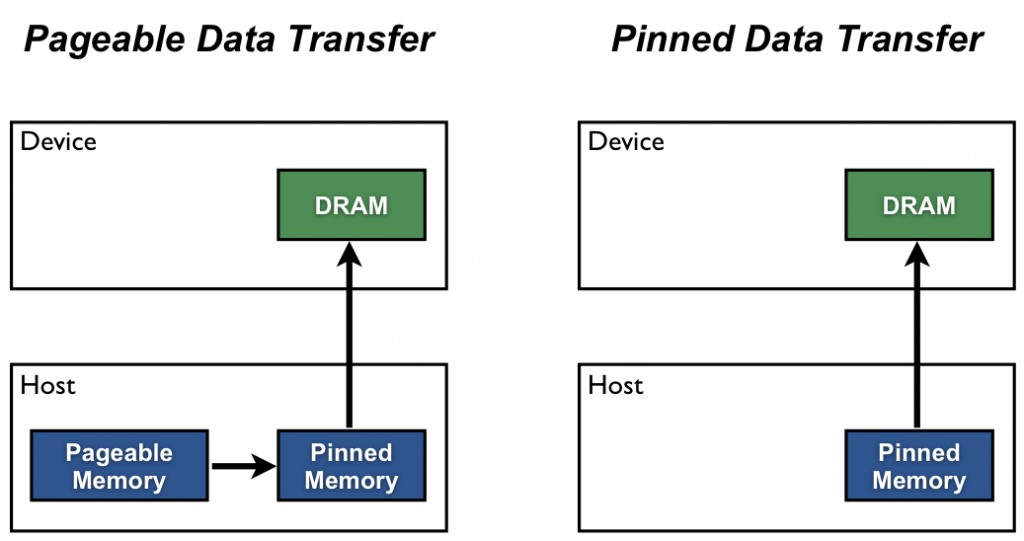
\includegraphics[scale=0.5]{images/pinning}
\caption[pinning]{GPU Data Transfers\cite{transfer}}
\end{figure}
Pinned memory is used as a straging area for transfers and we can avoid this cost by directly allocating our host arrays (e.g colours) in pinned memory.

Since we do not know the size of our 2D data arrays we will allocate all our data in normal memory using the standard library data structurs and then in a pre-processing stage call a \verb!pin_data! method on the mesh and similarly with the colours.
With extra code our data structures could be pinned straight away, however we perform this pre-processing stage as a comprimise to allow us to spend our time on GPU optimisations rather than speeding up the CPU code which does not count in the benchmark timings.

We can easily lift the code we will write for serializing data structures \verb!CUDATools.h! into the Mesh, so this should hopefully reduce time spent on this optimisation.